% datatrawl social card (GitHub repository preview) -- TikZ source of truth.
% Regenerate: make diagram
% 1280x640: two ghosted trawl nets flank a centered full mark, wordmark,
% letterspaced tagline, and repository URL. Mark from trawlmark.tikz.
\documentclass[tikz]{standalone}
\usetikzlibrary{calc}
% Shared trawl-net mark for the datatrawl brand assets.
%
% \input this file after \usetikzlibrary{...}; it provides two pics:
%   trawlmark  -- the full mark: ring, mesh, wake trails, incoming data
%                 dots, and the caught (ringed) node
%   trawlnet   -- ring + mesh only, inheriting the current draw color and
%                 opacity (the ghost/decoration variant)
% and the shared brand palette (cyA/cyB/cyC accents, ink, dim).
%
% Native coordinate frame: the 120x120 logo tile with y increasing DOWNWARD
% -- place pics inside a picture using [x=1pt, y=-1pt]. Mesh, wake, and dot
% tones are expressed with opacity rather than background color mixes, so
% the mark renders consistently on any of the asset backgrounds.
\definecolor{cyA}{HTML}{7df0e6}
\definecolor{cyB}{HTML}{34b8e0}
\definecolor{cyC}{HTML}{2bd4d4}
\definecolor{ink}{HTML}{e6f3fb}
\definecolor{dim}{HTML}{9fc2d6}

% One macro holds the net geometry; both pics call it. (Do NOT nest pics:
% transforms given as pic options reach the pic's own paths but not a
% nested \pic's -- discovered the hard way with a half-scaled mark.)
\newcommand{\trawlnetpaths}{%
    \draw[line width=2.4pt] (55,60) circle (42pt);
    \begin{scope}
      \clip (55,60) circle (41pt);
      \draw[line width=1.0pt, opacity=0.55]
        (13,44) .. controls (40,58) and (70,58) .. (97,44)
        (13,60) .. controls (40,74) and (70,74) .. (97,60)
        (13,76) .. controls (40,90) and (70,90) .. (97,76)
        (33,22) .. controls (43,55) and (43,65) .. (33,98)
        (55,18) .. controls (63,55) and (63,65) .. (55,102)
        (77,22) .. controls (83,55) and (83,65) .. (77,98);
    \end{scope}%
}

\tikzset{
  pics/trawlnet/.style={code={\trawlnetpaths}},
  pics/trawlmark/.style={code={
    % net (ring + mesh) in the accent blue
    \begin{scope}[cyB]
      \trawlnetpaths
    \end{scope}
    % wake trails behind the net
    \draw[cyB, opacity=0.35, line width=1.1pt]
      (58,112) .. controls (75,124) and (95,130) .. (120,132)
      (50,122) .. controls (68,136) and (92,144) .. (118,148)
      (62,132) .. controls (76,146) and (94,154) .. (112,158);
    % incoming data dots drifting toward the mouth of the net
    \fill[cyA]               (10,40) circle (2.0pt);
    \fill[cyA, opacity=0.80] (14,52) circle (1.6pt);
    \fill[cyA, opacity=0.65] ( 9,62) circle (1.4pt);
    \fill[cyA]               (16,69) circle (2.1pt);
    \fill[cyA, opacity=0.70] (12,79) circle (1.5pt);
    \fill[cyA, opacity=0.60] (19,46) circle (1.2pt);
    \fill[cyA, opacity=0.85] (21,60) circle (2.2pt);
    \fill[cyA, opacity=0.50] ( 8,55) circle (1.0pt);
    % the caught one, ringed
    \draw[cyC, line width=1.4pt] (96,40) circle (3.6pt);
    \fill[cyA]                   (96,40) circle (1.7pt);
  }},
}

\definecolor{cardtop}{HTML}{102f4c}
\definecolor{cardmid}{HTML}{0c2138}
\definecolor{cardbot}{HTML}{081320}
\definecolor{ghost}{HTML}{1f6f86}
\usepackage{lmodern}
\usepackage[T1]{fontenc}
\renewcommand{\familydefault}{\sfdefault}

\begin{document}
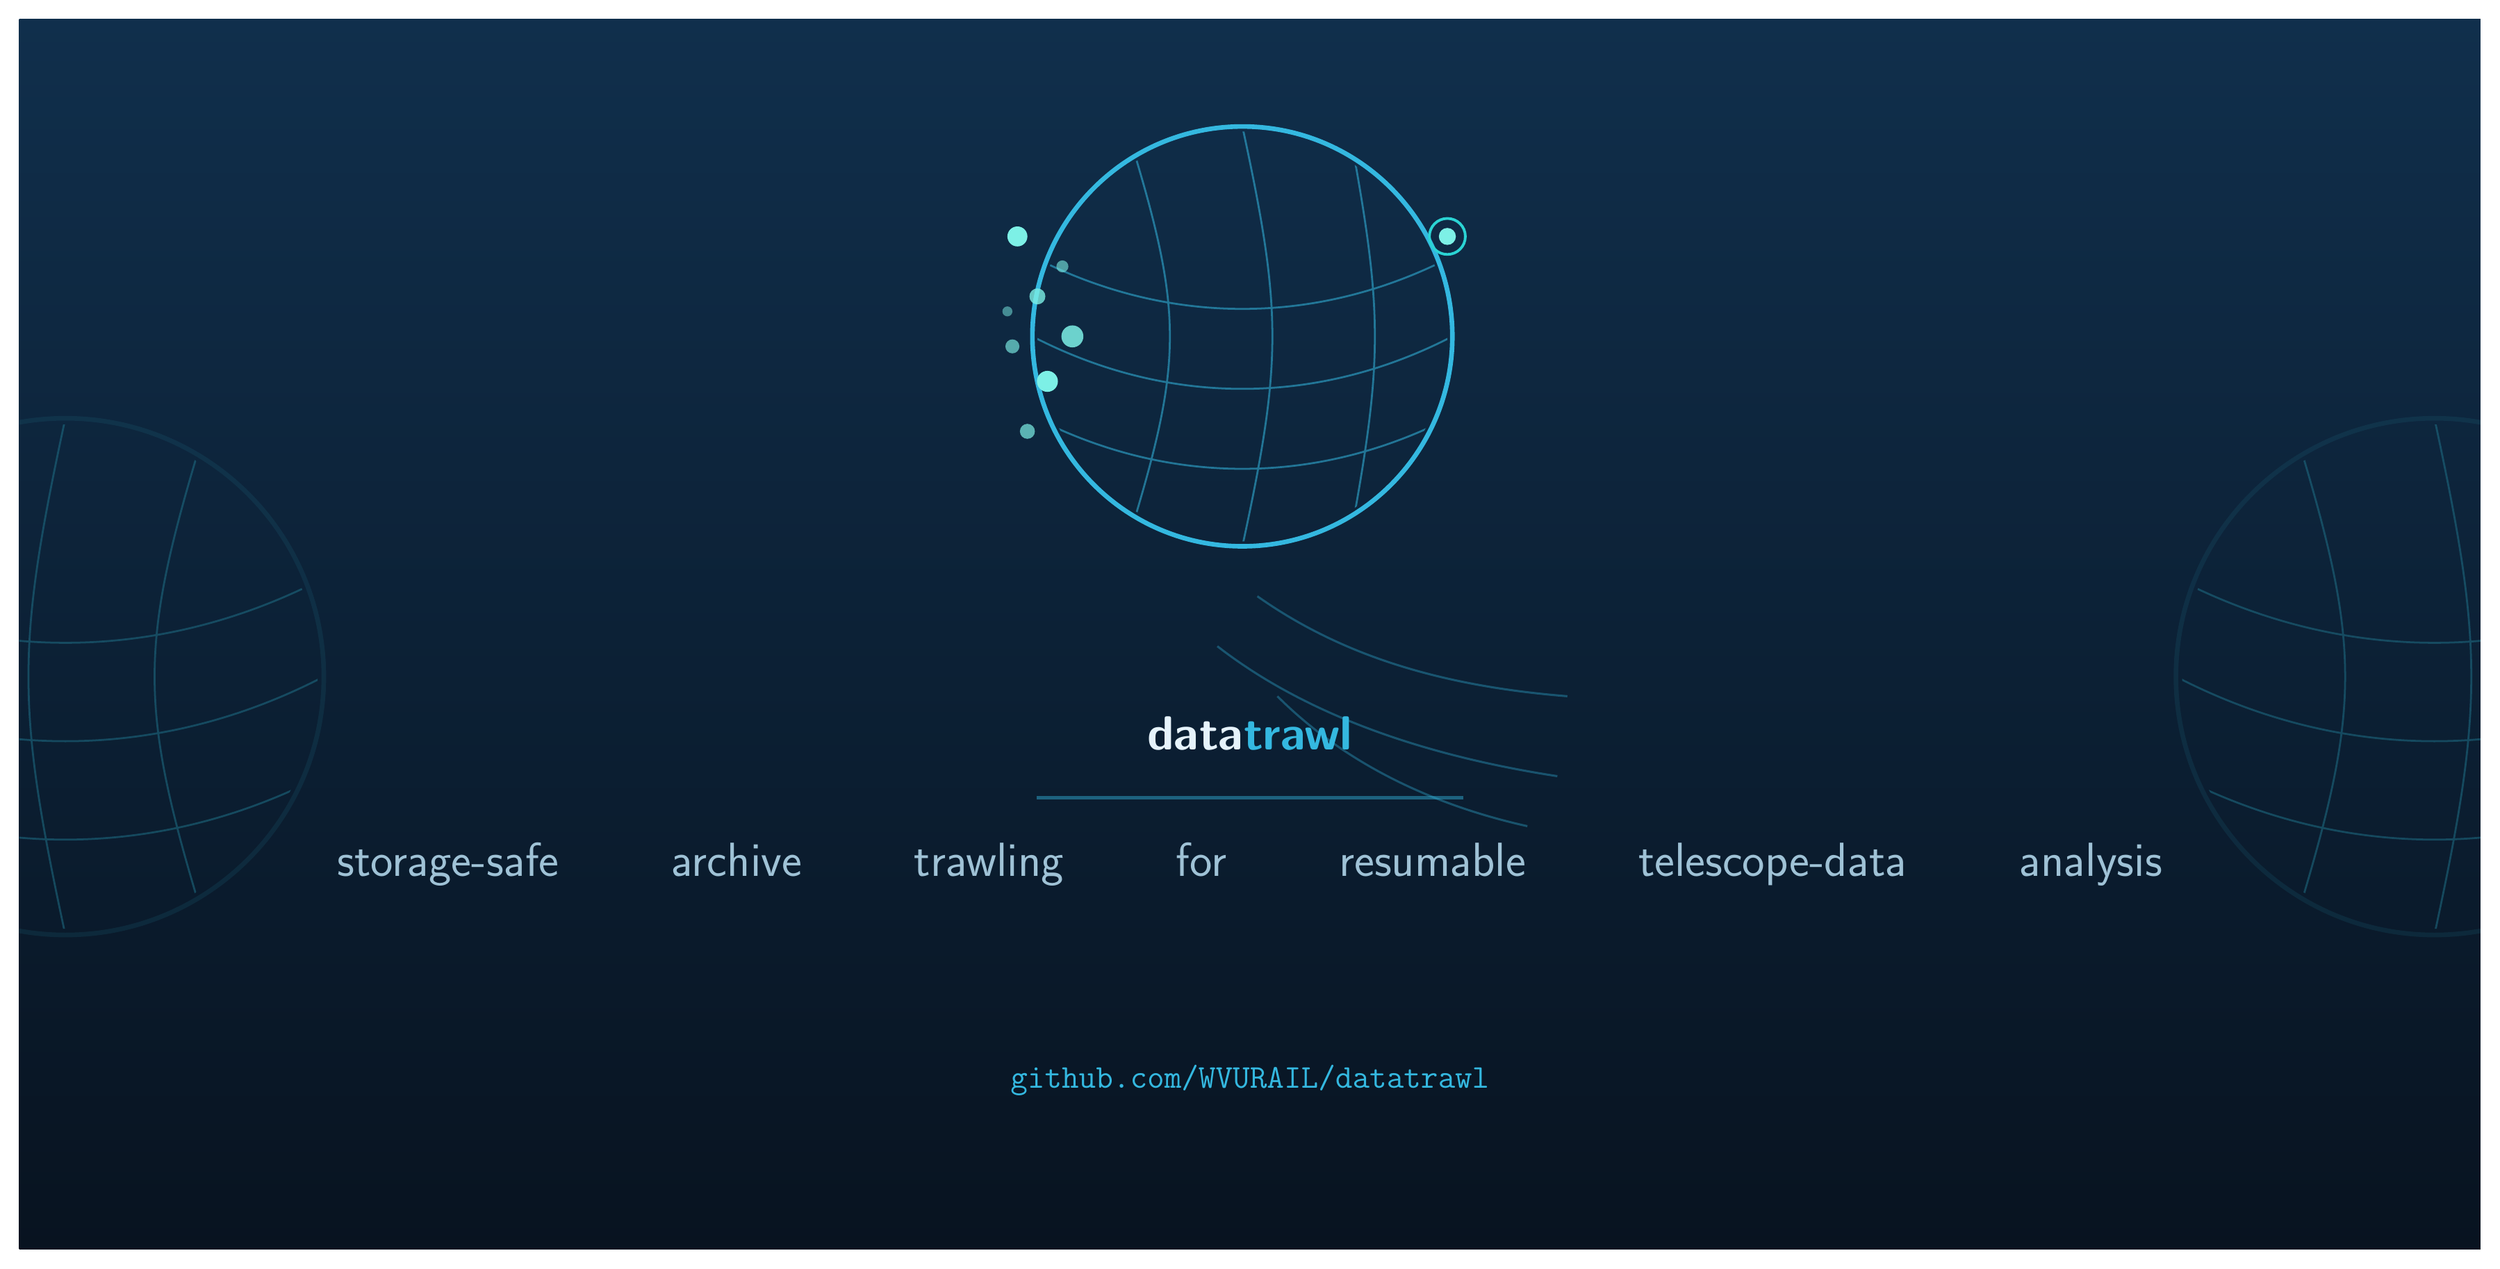
\begin{tikzpicture}[x=1pt, y=-1pt, every node/.style={inner sep=0pt}]

\shade[top color=cardtop, middle color=cardmid, bottom color=cardbot]
  (0,0) rectangle (1280,640);

% flanking ghost nets (left one mirrored, facing inward). Transformations
% must ride on the pic itself: an enclosing scope's scale does not reach a
% pic's path construction.
% clipped to the card: at 3.2x the nets overflow the canvas, and the
% standalone page would otherwise grow to fit them
\begin{scope}
  \clip (0,0) rectangle (1280,640);
  \pic[shift={(200,150)}, xscale=-3.2, yscale=3.2, ghost, opacity=0.18] {trawlnet};
  \pic[shift={(1080,150)}, scale=3.2, ghost, opacity=0.18] {trawlnet};
\end{scope}

% centered full mark
\pic[shift={(493.1,9)}, scale=2.6] {trawlmark};

% wordmark, two-tone as in the banner
\node[anchor=base] (wm) at (640,380)
  {\fontsize{107}{107}\selectfont\bfseries
   \textcolor{ink}{data}\textcolor{cyB}{trawl}};

% divider rule
\draw[cyB, opacity=0.45, line width=1.6pt] (529,405) -- (751,405);

% letterspaced tagline (stretched word gaps span the measured extent)
\node[anchor=base, text=dim] at (640,446)
  {\fontsize{23}{27}\selectfont\hbox to 949pt{storage-safe\hfil
   archive\hfil trawling\hfil for\hfil resumable\hfil
   telescope-data\hfil analysis}};

% repository URL
\node[anchor=base, text=cyB] at (640,556)
  {\fontsize{19}{22}\selectfont\ttfamily github.com/WVURAIL/datatrawl};

\end{tikzpicture}
\end{document}
